\section{Vorbereitungsfragen}
\label{sec:Vorbereitungsfragen}

\subsection{Aufbau und Wirkungsweise der Brennstoffzelle am Beispiel der PEMFC}
In \autoref{fig:230618_PEMFC_Aufbau} ist der Aufbau einer üblichen PEM-Brennstoffzelle veranschaulicht. 
Eine PEMFC ist eine Brennstoffzelle, die Wasserstoff und Sauerstoff in elektrische Energie umwandelt.
Dabei wird Wasserstoff auf der Oberfläche der Anode unter Elektronenabgabe oxidiert.
Die Wasserstoffprotonen wandern durch die Membran zur Kathode.
Die Elektronen fließen durch einen äußeren Stromkreis und erzeugen dabei elektrische Energie.
An der Kathode werden die Elektronen mit den Wasserstoffprotonen und Sauerstoff Atomen reduziert und bilden Wasser.

\begin{figure}[H]
    \centering
    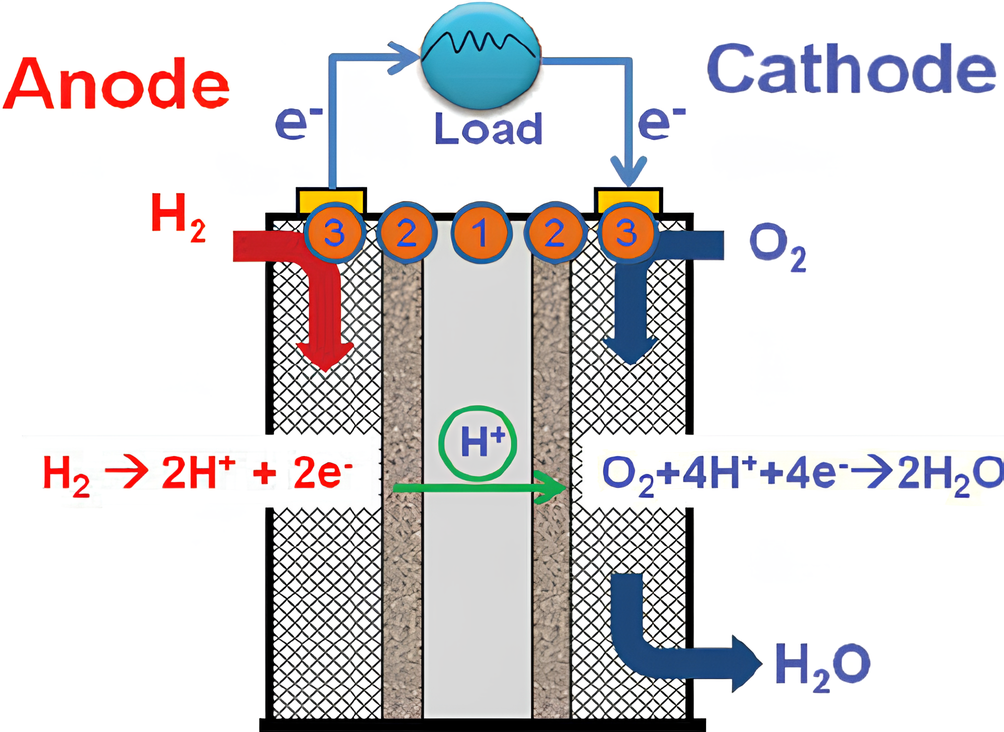
\includegraphics[width=0.5\textwidth]{Abbildungen/PEMFC_Aufbau.png}
    \caption{Aufbau und Funktionsweise einer PEMFC \cite{PEMFC}}
    \label{fig:230618_PEMFC_Aufbau}
\end{figure}

\subsection{Ausführungsformen von Brennstoffzellen}

\begin{table}[H]
    \caption{Ausführungsformen von Brennstoffzellen}
    \centering
        \begin{tabular}[pos]{|c|c|c|c|c|c|}
            \hline
            \rowcolor[HTML]{70AD47} 
            BZ-Typen    & Elektrolyt                        & Brennstoff                        & Oxidator                  & Arbeitstemp.          & $\eta$            \\
            \rowcolor[HTML]{70AD47} 
                        &                                   & (Anode)                           & Kathode                   & in °C                 &                   \\\hline\hline
            AFC         & 30\%'ige                          & nur reinst                        & nur reinst                & 60 - 80               & $70 - 75\%$       \\
                        & KOH-Lauge                         & $H_2$                             & $O_2$                     &                       &                   \\\hline
            PEMFC       & PEM (z.B. Nafion)                 & $H_2$,                            & $O_2$, Luft               & 70 - 90               & $40 - 50\%$       \\
                        &                                   & Reformat gas                      &                           &                       &                   \\\hline
            DMFC        & PEM (z.B. Nafion)                 & $CH_3OH$                          & $O_2$, Luft               & 60 - 120              & $40\%$            \\\hline
            PAFC        & Phosphorsäure                     & $H_2$, $CH_4$,                    & $O_2$, Luft               & 170 - 200             & $40 - 50\%$       \\
                        &                                   & Sondergase                        &                           &                       &                   \\\hline
            MCFC        & Akalicarbonat-                    & $H_2$, Erdgase                    & $O_2$, Luft               & 650                   & $55 - 60\%$       \\
                        & schmelzen                         & Sondergase                        &                           &                       &                   \\\hline
            SOFC        & Ytriumdotiertes-                  & $H_2$, Erdgas,                    & $O_2$, Luft               & 900 - 1000            & $60 - 70\%$       \\
                        & zirkonoxod                        & Sondergase                        &                           &                       &                   \\\hline
        \end{tabular}
        \label{tab:20230618_BZ-arten}
\end{table}

\subsection{Skizzieren Sie qualitativ die U-I-Kennlinie einer Brennstoffzelle und erläutern Sie Arbeitsbereiche und markante Betriebsparameter}

\begin{figure}[H]
    \centering
    \includegraphics[width=0.8\textwidth]{Abbildungen/U-I-Kennlinie.png}
    \caption{U-J Kennlinie einer Brennstoffzelle vgl. \cite{BZ-Folien}}
    \label{fig:230618_U-I-Kennlinie}
\end{figure}

In \autoref{fig:230618_U-I-Kennlinie} ist eine Skizze der U-J Kennlinie einer Brennstoffzelle zu erkennen.
Durch die Proportionalität zwischen Stromdichte und der Stromstärke ist das qualitative Aussehen der U-I und der U-J Kennlinie deckungsgleich.
Die markierten Bereiche unterscheiden sich jeweils durch die vorherrschenden Verluste.
In Bereich 1 sind die Aktivierungsverluste maßgeblich, da eine Energiebarriere der Reaktion überwunden werden muss.
Im 2. Bereich dominieren die Ohm'schen Verluste, die aufgrund des Transports der Ionen durch den Elektrolyten und der Elektronen durch das Elektrodenmaterial auftreten.
Im Bereich 3 wird die Reaktion durch die Diffusionsfähigkeit der Gase und der Elektrodenstruktur bestimmt.

\subsection{Die Faraday'schen Gesetze.}

\subsubsection{1. Faraday'sches Gesetz}

Die Stoffmenge($n$), die an einer Elektrode während der Elektrolyse abgeschieden wird, ist proportional zur Ladung($Q$), die durch den Elektrolyten geschickt wird \cite{Faraday_G} und beschreibt somit die \autoref{eq:230618_1FaradayGesetz}.
Die heutige Formulierung berücksichtigt verschiedene Umformungen und die Wertigkeit des Ions (\autoref{eq:230618_1FaradayGesetz_Heute}).

\begin{equation}
    n \sim Q
    \label{eq:230618_1FaradayGesetz}
\end{equation}

\begin{equation}
    Q = n \cdot z \cdot F
    \label{eq:230618_1FaradayGesetz_Heute}
\end{equation}

\subsubsection{2. Faraday'sches Gesetz}

Die durch eine bestimmte Ladung abgeschiedene Masse eines Elements ist proportional zum Atomgewicht des abgeschiedenen Elements und umgekehrt proportional zu seiner Wertigkeit, daher zur Anzahl von einwertigen Atomen, die sich mit diesem Element verbinden können \cite{Faraday_G}. Das entspricht \autoref{eq:230618_2FaradayGesetz}.
Heutzutage wird das 2. Faraday'sche Gesetz mit \autoref{eq:230618_2FaradayGesetz_Heute} Formuliert.

\begin{equation}
    m \sim \frac{M}{z}
    \label{eq:230618_2FaradayGesetz}
\end{equation}

\begin{equation}
    m = M \cdot n = \frac{M \cdot Q}{z \cdot F} = \frac{M \cdot I \cdot t}{z \cdot F}
    \label{eq:230618_2FaradayGesetz_Heute}
\end{equation}

\subsection{Herleitung des Umsatzwirkungsgrads}

Der Faraday'sche Wirkungsgrad lässt sich nach \autoref{eq:230618_Faraday-Wirkungsgrad} aus dem Quotienten von theoretisch benötigtem Wasserstoffvolumen und dem tatsächlich benötigtem gemessenen verbrauchtem Wasserstoff ermitteln.
Das theoretisch benötigte Wasserstoffvolumen lässt sich mittels \autoref{eq:230618_Volumen-H2-Theoretisch} berechnen und entspricht einer umgeformten \autoref{eq:230618_2FaradayGesetz_Heute}.

\begin{equation}
    \eta_{Theor.} = \frac{V_{Theoretisch(H_2)}}{V_{Praktisch(H_2)}}
    \label{eq:230618_Faraday-Wirkungsgrad}
\end{equation}

\begin{equation}
    V_{H_2} = \frac{I \cdot t \cdot V_m}{z \cdot F}
    \label{eq:230618_Volumen-H2-Theoretisch}
\end{equation}

\subsection{Der elektroenergetische Wirkungsgrad}

Der elektroenergetische Wirkungsgrad berechnet sich aus gewonnener elektrischer Energie und der verbrauchten chemischen Energie nach \autoref{eq:230619_Elektroenergetisch} \cite{BZ-Folien}.

\begin{equation}
    \eta_{Energetisch} = \frac{E_{Elektrisch}}{E_{Chemie}} = \frac{U \cdot I \cdot t}{\Delta H_{(H_2)} \cdot V_{Praktisch}}
    \label{eq:230619_Elektroenergetisch}
\end{equation}

\subsection{Gleichgewichtsspannung und Thermoneutralspannung bei Standardbedingungen}

Standardbedingungen beschreiben in diesem Fall den Normaldruck von $1015mBar$, eine Luftfeuchte von $0\%$ und eine Umgebungstemperatur von 25°C.
Die Thermoneutrale Spannung stellt hier die maximal erreichbare Spannung einer einzelnen Brennstoffzelle dar und beläuft sich bei Standardbedingungen auf $U_{th} = 1,48V$, 
die Gleichgewichtsspannung hingegen ist die elektrisch maximal nutzbare Spannung und beträgt bei Standardbedingungen $U_0 = 1,23V$ die Differenz zwischen der Thermoneutralen und der Gleichgewichtsspannung lässt sich auf die Entropie des Wassers zurückführen.   

\subsection{Berechnen Sie für den Prozesstemperaturbereich von 0°C bis etwa 1500 °C bei 25°C
Umgebungstemperatur den Carnot-Wirkungsgrad und den Gibbs-Helmholtz-Wirkungsgrad
und stellen Sie beide Verläufe in einem Bild grafisch dar! Zur Erleichterung sei auf den
linearen Enthalpie verlauf hingewiesen.}

Die Wirkungsgrade lassen sich mittels der Gleichungen \ref{eq:230620_Carnot} und \ref{eq:230620_Gibbs-Helmholtz} berechnen. 
$T_{Unten}$ bezeichnet die niedrigere Temperatur im Prozess, $T_{Oben}$ die höhere, $\Delta G_R$ ist die freie Reaktionsenthalpie und $\Delta H_R$ die Enthalpie des Wassers.
Zur numerischen Ermittlung der Enthalpien wird die beigelegte Grafik und das Programm PowerToys - Bildschirmlineal verwendet.
Damit werden genaue Pixel-Abstände zwischen den Linien bestimmt und zu den gegeben Einheit umgerechnet.
Es werden damit folgende Eckdaten ermittelt:
\begin{align}
    \Delta G_R(300K) &= 227 \frac{kJ}{mol} \nonumber\\
    \Delta G_R(373K) &= 212 \frac{kJ}{mol} \nonumber\\
    \Delta G_R(1100K) &= 167 \frac{kJ}{mol} \nonumber\\
    \Delta H_R(T) &= 
        \begin{cases}
            286 \frac{kJ}{mol}, & T < 373 K \\
            246 \frac{kJ}{mol}, & T \geq 373 K
        \end{cases} \nonumber
\end{align}

Durch diese Punkte können für $\Delta G_R$ 2 lineare Gleichungen aufgestellt werden, welche sich zu \autoref{eq:230620_d_G_R} kombinieren lassen.

\begin{equation}
    \Delta G_R(T) =
    \begin{cases}
        -0,2055 \cdot T + 288,6438 K, & T < 373 K \\
        -0,0619 \cdot T + 235,0880 K, & T \geq 373 K
    \end{cases}
    \label{eq:230620_d_G_R}
\end{equation}

\begin{equation}
    \eta_{Carnot} = 1 - \frac{T_{Unten}}{T_{Oben}}
    \label{eq:230620_Carnot}
\end{equation}

\begin{equation}
    \eta_{th} = \frac{\Delta G_R}{\Delta H_R}
    \label{eq:230620_Gibbs-Helmholtz}
\end{equation}

Die errechneten Werte können nun mittels Matlab in \autoref{fig:230620_Enthalpie} und \autoref{fig:230620_Wirkungsgrade} dargestellt werden.

\begin{figure}[H]
    \centering
    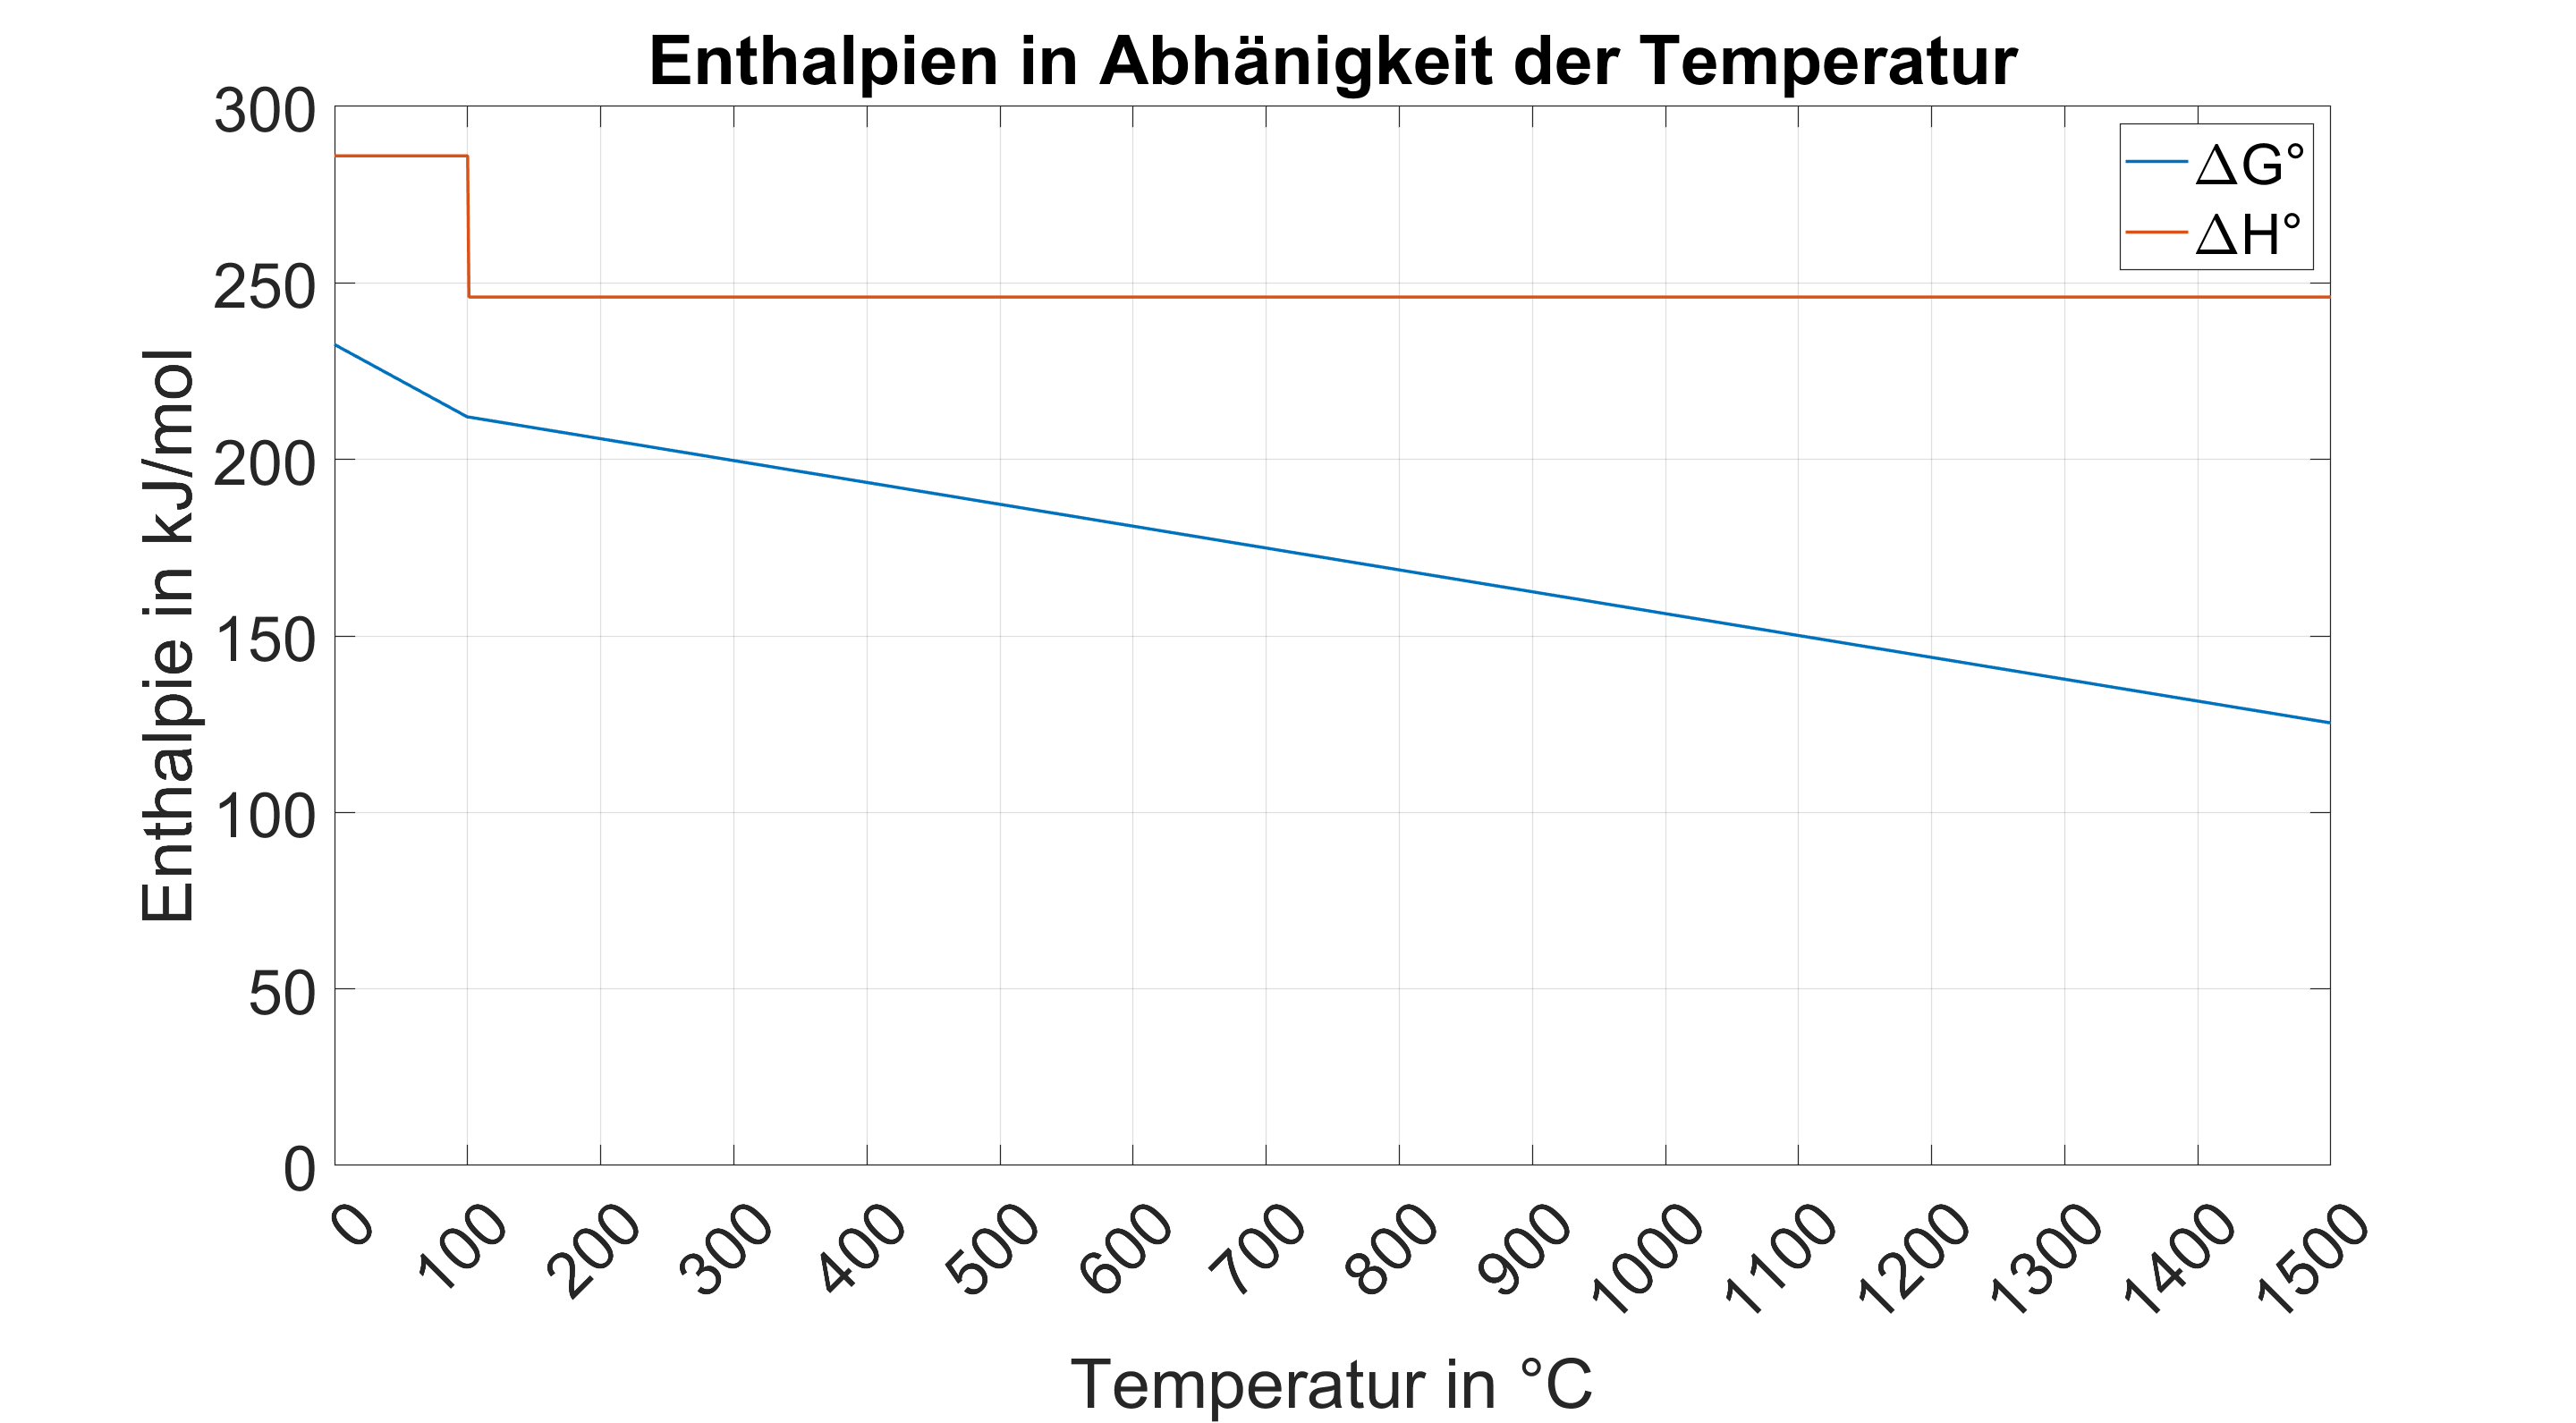
\includegraphics[width=\textwidth]{Abbildungen/Enthalpien.png}
    \caption{Freie Standardenthalpie und Enthalpie von Wasser über der Temperatur}
    \label{fig:230620_Enthalpie}
\end{figure}

\begin{figure}[H]
    \centering
    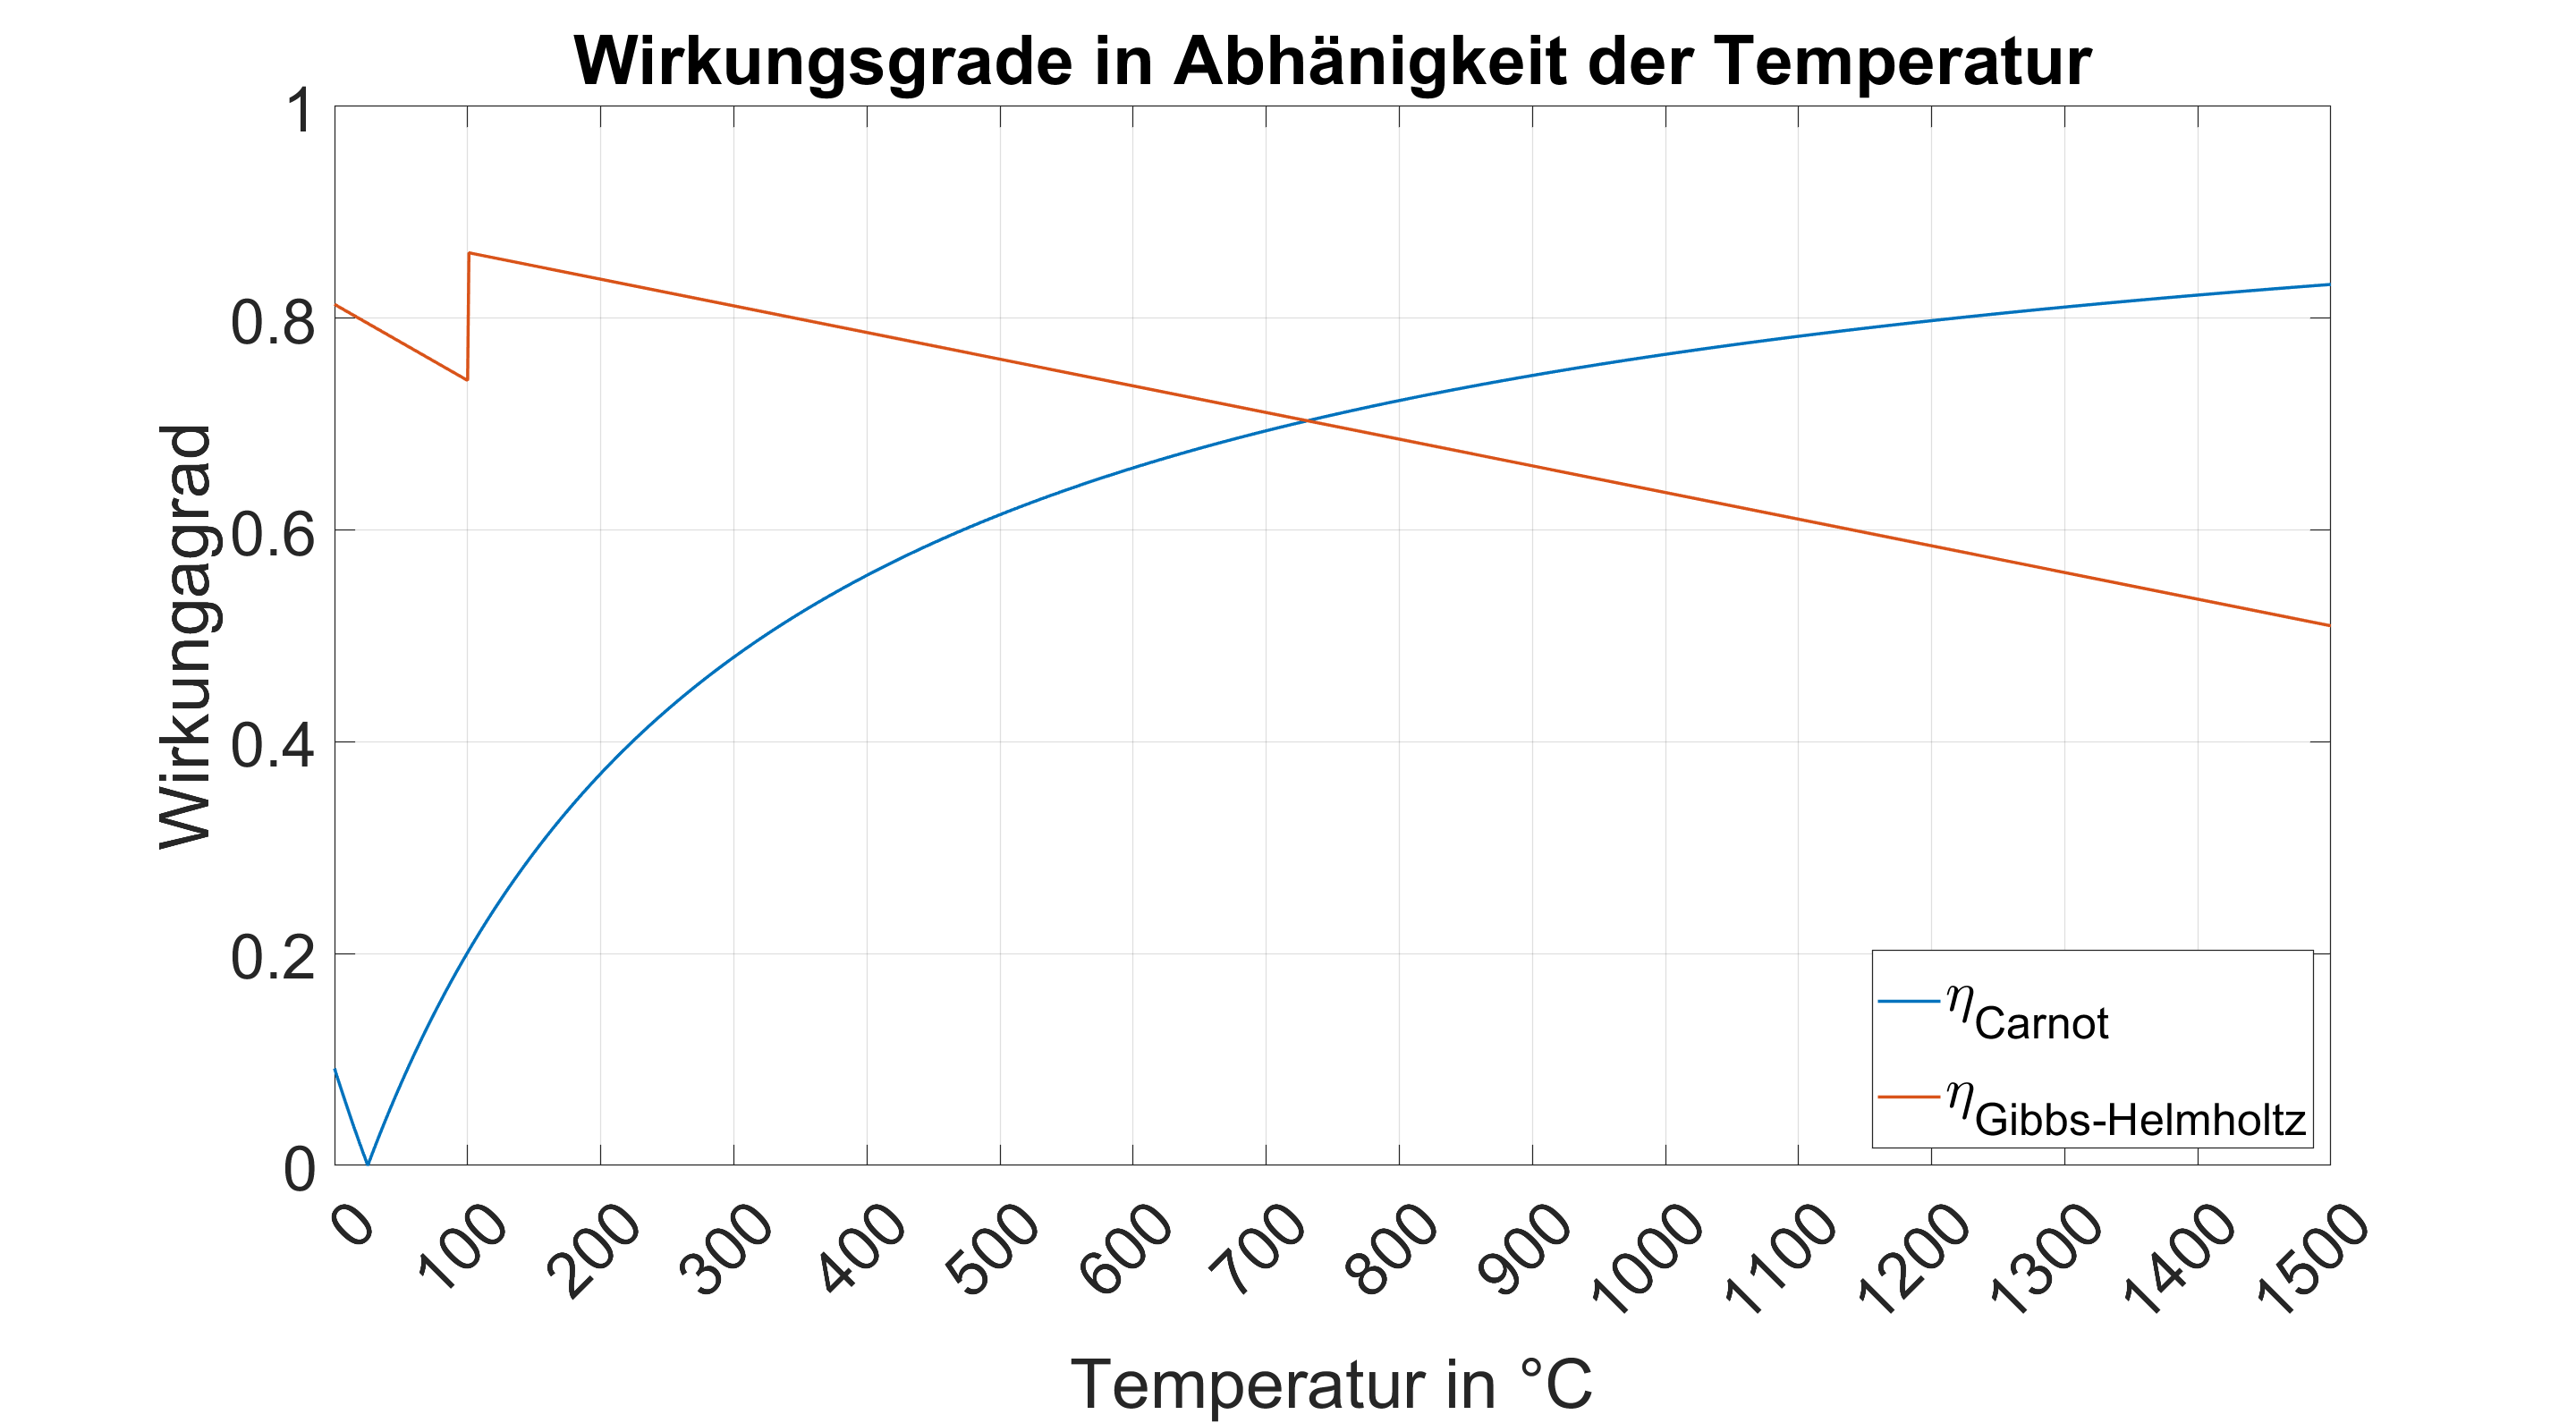
\includegraphics[width=\textwidth]{Abbildungen/Wirkungsgrade.png}
    \caption{Carnot-Wirkungsgrad und Gibbs-Helmholtz-Wirkungsgrad über der Temperatur}
    \label{fig:230620_Wirkungsgrade}
\end{figure}

\subsection{Vergleich thermische Energiesysteme mit Brennstoffzellensystemen}

Thermische Energiesysteme haben im Allgemeinen einen geringeren Wirkungsgrad als Brennstoffzellensysteme, da sie  mehr Energieumwandlungen durchlaufen müssen:
$$E_{Chemisch} \Rightarrow E_{Thermisch} \Rightarrow E_{Mechanisch} \Rightarrow E_{Elektrisch}$$ 
Brennstoffzellensysteme durchgehen aufgrund der kalten Verbrennung nur eine Umwandlung:
$$E_{Chemisch} \Rightarrow E_{Elektrisch}$$

Jeder der Pfeile ist mit einem Wirkungsgrad und dadurch mit Verlusten verbunden.

\subsection{Ermitteln Sie für einen 1,2 kW-Brennstoffzellen Stack, der in einem 24-V-System mit
BleiGel Batteriepuffer im Nennbetrieb arbeitet, die stündlich entstehende Wassermenge.
Während eines Volladezyklus schwankt die BZ-Zellspannung zwischen 1 und 0,6 Volt.}
\label{sec:VF_H2O_Menge}

Zunächst muss mit \autoref{eq:230620_n_Zelle} die mögliche anzahl an Brennstoffzellen berechnet werden.

\begin{equation}
    n_{Zellen} = \frac{U_{System}}{U_{Zelle}}\\
    \label{eq:230620_n_Zelle}
\end{equation}

\begin{align}
    n_{Zelle,Min} &= \frac{24V}{1V} = 24 \nonumber\\
    n_{Zelle,Max} &= \frac{24V}{0.6V} = 40 \nonumber
\end{align}

Anschließend kann mit \autoref{eq:230620_Wassermenge} (den Faraday'schen Gesetzen) die entstehende Wassermenge bzw. der Massenstrom des Wassers berechnet werden.
Hierbei wird von einer molaren Masse für Wasser von $M_{Wasser} = 18 \cdot 10^{-3} \frac{kg}{mol}$ und der Faradaykonstante von $F =96485,33 \frac{A\cdot s}{mol}$ ausgegangen.

\begin{equation}
    m = \frac{M \cdot I \cdot t}{z \cdot F} \Leftrightarrow \frac{m}{t} = \dot{m} = \frac{M \cdot \frac{P_{System}}{U_{System}}}{z \cdot F} \cdot 3600 \frac{s}{h}
    \label{eq:230620_Wassermenge}
\end{equation}

$$\dot{m}_{Zelle} = 0,403 \frac{kg}{h}$$

Durch die Multiplikation mit der Zellenanzahl ergibt sich damit die Wassermenge für den gesamten Brennstoffzellenstack in einer Stunde, wie in Gleichung \autoref{eq:230620_gesamt_Wassermenge} veranschaulicht.

\begin{equation}
    \dot{m}_{gesamt} = \dot{m}_{Zelle} \cdot n_{Zelle}
    \label{eq:230620_gesamt_Wassermenge}
\end{equation}
\begin{align}
    \dot{m}_{gesamt,Min} &= \dot{m}_{Zelle} \cdot n_{Zelle,Min} = 0,403 \frac{kg}{h} \cdot 24 = 9,672 \frac{kg}{h} \nonumber\\
    \dot{m}_{gesamt,Max} &= \dot{m}_{Zelle} \cdot n_{Zelle,Max} = 0,403 \frac{kg}{h} \cdot 40 = 16,12 \frac{kg}{h} \nonumber\\
    \dot{m}_{gesamt} &= (9,672 \dots 16,12) \frac{kg}{h} \nonumber
\end{align}

\subsection{Der Stack von \ref{sec:VF_H2O_Menge} verbraucht bei Nennstrom stündlich 904 Liter Wasserstoff (Messung bei 24°C (= 297,15 K) und 1018mbar (= 101,8 kPa) äußerem Luftdruck). 
Bestimmen und kommentieren Sie den Faraday'schen Wirkungsgrad. Wie groß ist der elektroenergetische Wirkungsgrad?}

% \textcolor{red}{\Huge Faraday Wirkungsgrad ergibt unsinnige Werte}

Zunächst muss das molare Volumen von Wasserstoff bei angegebenen Druck und Temperaturen ermittelt werden.
Dazu wird die spezielle Gaskonstante von Wasserstoff als $R_{i,H_2} = 8,3144 \frac{kPa \cdot l}{mol \cdot K}$ \cite{Gaskonstante} angenommen.
Mittels \autoref{eq:230624_Molaresvolumen} kann das molare Volumen von $V_m = 24,2694 \frac{l}{mol}$ bestimmt werden.
Durch das Umstellen des 2. Faraday'schen Gesetz aus \autoref{eq:230618_Volumen-H2-Theoretisch} kann man den theoretisch benötigten Wasserstoff Volumenstrom berechnen, wie in \autoref{eq:230624_Volumenstrom-theor} angegeben.
Mit einem Strom von $I = 50A$, $z = 2$ und der Faradaykonstante von $F = 96485,33 \frac{A \cdot s}{mol}$, ergibt sich ein theoretisch benötigter Wasserstoff Volumenstrom von $\dot{V}_{H_2,Theor.} = 22,6381 \frac{l}{h}$.
Dieser Volumenstrom bezieht sich jedoch nur auf eine einzelne Brennstoffzelle und muss nun auf den gesamten Stack hochgerechnet werden.
Abweichend zu \autoref{sec:VF_H2O_Menge} wird hier von einer mittleren Spannung ausgegangen, welche sich auf $U_{Zelle} = 0,8V$ beläuft und somit eine Zellenanzahl $n_{Zellen} = 30$ angibt.
Mit \autoref{eq:230624_Faraday-Wirkungsgrad} ergibt sich der Faraday´sche Wirkungsgrad von $\eta_{Faraday} = 75,13 \%$


\begin{equation}
    V_m = \frac{R_{i,H_2} \cdot T}{p}
    \label{eq:230624_Molaresvolumen}
\end{equation}

\begin{equation}
    V_{H_2,Theor.} = \frac{I \cdot t \cdot V_m}{z \cdot F} \Leftrightarrow  \dot{V}_{H_2,Theor.} = \frac{I \cdot V_m}{z \cdot F}
    \label{eq:230624_Volumenstrom-theor}
\end{equation}

$$\dot{V}_{H_2,Theor.} = \frac{50 A \cdot 24,2694 \frac{l}{mol}}{2 \cdot F}= 22,6381 \frac{l}{h}$$

\begin{equation}
    \eta_{Faraday} = \frac{n_{Zelle} \cdot \dot{V}_{H_2,Theor.}}{\dot{V}_{H_2}}
    \label{eq:230624_Faraday-Wirkungsgrad}
\end{equation}

$$\eta_{Faraday} = \frac{30 \cdot 22,6381 \frac{l}{h}}{904 \frac{l}{h}}= 0,7513=75,13\%$$


Der elektroenergetische Wikrungsgrad lässt sich mithilfe der \autoref{eq:230619_Elektroenergetisch} berechnen.
Hierbei wird der Term $\frac{t}{V_{Praktisch}}$ zu $\frac{1}{\dot{V}_{Praktisch}}$ umgeformt und die Spannung mit der Anzahl der Zellen multipliziert.
Der Brennwert von Wasserstoff wird als $\Delta H_{H_2} = 3,54\frac{Wh}{l}$ \cite{dH-H2} angenommen.
Daraus ergibt sich ein elektroenergetischer Wirkungsgrad von $\eta_{Elektroenergetisch} = 0,374981 \equiv 37,4981 \%$.

$$\eta_{Energetisch} = \frac{(0,8V \cdot 30) \cdot 50A}{3,54 \frac{Wh}{l} \cdot 904 \frac{l}{h}}=0,3749=37,49 \%$$

\subsection{Berechnung der Wärmeentwicklung an der Brennstoffzelle im Betriebsfall}

Näherungsweise kann der thermische Wirkungsgrad als $\eta_{Thermisch} = 1 - \eta_{Elektroenergetisch} = 62,5019 \%$.
Mit \autoref{eq:230624_Wärmeleistung} und der angegebenen Leistung aus \autoref{sec:VF_H2O_Menge} ergibt sich eine Wärmeleistung von $P_{Wärme} = 750,023 W$. 

\begin{equation}
    P_{W"arme} = \eta_{Thermisch} \cdot P_{Elektrisch}
    \label{eq:230624_Wärmeleistung}
\end{equation}

\subsection{Wie groß ist der elektrische Wirkungsgrad, wenn der Stack eine Wärmeleistung von
230W produziert und bei einer Spannung von 42V ein Strom von 10 A entnommen werden kann?}

Der elektrische Wirkungsgrad lässt sich durch den Quotienten aus elektrischer Leistung und der Gesamtleistung berechnen, was in \autoref{eq:230624_el-Wirkungsgrad} dargestellt wird. 
Die elektrische Leistung beläuft sich nach \autoref{eq:230624_El-Leistung} auf $P_{El} = 420W$. Somit ergibt der elektrische Wirkungsgrad $\eta_{El} = 64,6\%$

\begin{equation}
    P_{El} = U \cdot I
    \label{eq:230624_El-Leistung}
\end{equation}

$$P_{EL} = 42V \cdot 10A = 420W$$

\begin{equation}
    \eta_{El} = \frac{P_{El}}{P_{El} + P_{Wärme}} 
    \label{eq:230624_el-Wirkungsgrad}
\end{equation}

$$\eta_{El}= \frac{420 W}{420 W + 230 W} = 0,646 \equiv 64,6 \%$$